% Goes in previous section: In lattice QCD, we represent quark fields directly as Grassmann-valued fields on spacetime lattice sites, but we represent gluon fields as discretized gauge-transporters called \textit{link variables}, which are envisaged as directional links between lattice sites. (Gatt. and Lang pg. 34-35)
\section{Basic Building Blocks}
    Quarks and gluons are the principal objects of quantum chromodynamics, and form the hadrons which we wish to study. Hence, the operators we use to create hadrons on the lattice are constructed using building blocks of quark and gluon fields. Since hadrons are not point-like objects, but extended composite objects, we form our hadron operators out of \textit{covariantly-displaced} quark fields. In calculating correlation functions (\emph{correlators}) on the lattice, two important obstacles must be confronted:  noise, and excited-state contamination (contributions to correlators from higher-lying states than those we wish to study). With these challenges in mind, our basic building blocks are so-called \textit{stout-smeared}~\cite{Morningstar:2003gk} gauge-link field variables and \textit{LapH-smeared}~\cite{Peardon:2009gh, Morningstar:2011ka} quark field variables. We will see that the stout smearing procedure leads to dramatically reduced noise in the evaluation of correlators constructed with displaced operators, and that the LapH-smearing procedure drastically attenuates contributions from higher-lying modes of the theory. Both of these procedures are crucial for extracting the energy spectrum, as we will see in Chapter~\ref{ch:analysis}.
    \subsection{Stout Smearing}
    In order to combat excited-state contamination, we must design operators which couple more to the low-lying states of interest, rather than excited states. When examining states containing gluons, such as glueballs or hybrid mesons, a way to reduce excited-state contamination is by the use of gauge-link smearing. Ref.~\cite{Morningstar:2003gk} describes a smearing procedure for link variables known as stout smearing, which is outlined here. We will see that even when we are not interested in extracting gluonic states, gauge-link smearing helps to attenuate noise in extracting hadronic observables from the lattice.
    
    Define $C_\mu(x)$ as the following weighted sum of perpendicular link-variable staples (depicted in Figure~\ref{fig:staples}) beginning at a lattice site $x$ and terminating at a neighboring site $x + \hat\mu$,
    \begin{equation}\label{eq:staples}
        C_{\mu}(x)= \sum_{\nu \neq \mu} \rho_{\mu \nu}\left(U_{\nu}(x) U_{\mu}(x+\hat{\nu}) U_{\nu}^{\dagger}(x+\hat{\mu})\right.\left.+U_{\nu}^{\dagger}(x-\hat{\nu}) U_{\mu}(x-\hat{\nu}) U_{\nu}(x-\hat{\nu}+\hat{\mu})\right),
    \end{equation}
    where $\rho_{\mu\nu}$ are tunable real parameters, and $\hat\mu$ and $\hat\nu$ are unit vectors on the lattice. We use the following weights,
    \begin{equation}
        \rho_{j k}=\rho, \quad \rho_{4 \mu}=\rho_{\mu 4}=0,
    \end{equation}
    which amount to smearing spacial link variables only.
    % To do: make note of positive definiteness, add bits about parameters we use.
    Next, define a matrix $Q_\mu(x)$ in SU($N$) by
    \begin{equation}
        \begin{aligned}
            Q_{\mu}(x)&=\frac{i}{2}\left(\Omega_{\mu}^{\dagger}(x)-\Omega_{\mu}(x)\right)-\frac{i}{2 N} \operatorname{Tr}\left(\Omega_{\mu}^{\dagger}(x)-\Omega_{\mu}(x)\right), \text{ where}\\
            \Omega_{\mu}(x)&=C_{\mu}(x) U_{\mu}^{\dagger}(x)  \quad \text { (no summation over } \mu).
        \end{aligned}
    \end{equation}
    Being both Hermitian and traceless, $Q_\mu(x)$ is also in the Lie algebra $\mathfrak{su}(N)$, and therefore $e^{iQ_\mu(x)} \in \mathrm{SU}(N)$. Then define an iterative process whereby a link variable at step $n + 1$ is related to a link variable at step $n$ as,
    \begin{equation}
        U_{\mu}^{(n+1)}(x)=\exp \left(i Q_{\mu}^{(n)}(x)\right) U_{\mu}^{(n)}(x).
    \end{equation}
    Since the link variables we start with are in SU($N$) and so is $e^{iQ_\mu(x)}$, we guarantee that each link variable in this iteration is also in SU($N$). This ensures that transforming the link variables in this way preserves the property that they are members of the SU(3) gauge group.
    \begin{figure}
        \centering
        \begin{tikzpicture}
            \draw [very thick, dashed, -Latex] (0,0) -- (0.7,0);
            \draw [very thick, dashed] (0.5,0) -- (1,0);
            \draw (0.5, -0.5) node {\small$C_\mu(x)$};
            % \draw (0,0.3) node {\small$x$};
            % \draw (1,0.3) node {\small$x+\mu$};
            \draw (2,0) node {$=$};
            % \draw [very thick,-Latex] (0,0) -- (1.75,0);
            % \draw [very thick] (1.5,0) -- (3,0);
            % \draw (1.5,-1.1) node {\small $U_{\mu}(n)$};
            % \draw [very thick] (7,0) -- (8.65,0);
            % \draw [very thick,Latex-] (8.3,0) -- (10,0);
            % \draw (8.7,-1.1) node {\small$U_{-\mu}(n)= U_\mu^\dagger(n-\hat\mu)$};
            \draw [very thick,-Latex] (3,-0.5) -- (3,0.2);
            \draw [very thick] (3,0) -- (3,0.5);
            \draw [very thick,-Latex] (3,0.5) -- (3.7,0.5);
            \draw [very thick] (3.5,0.5) -- (4,0.5);
            \draw [very thick,-Latex] (4,0.5) -- (4,-0.2);
            \draw [very thick] (4,0) -- (4,-0.5);
            % \draw (3,-0.8) node {\small$x$};
            % \draw (4,-0.8) node {\small$x+\mu$};

            \draw (5,0) node {$+$};

            \draw [very thick,-Latex] (6,0.5) -- (6,-0.2);
            \draw [very thick] (6,0) -- (6,-0.5);
            \draw [very thick,-Latex] (6,-0.5) -- (6.7,-0.5);
            \draw [very thick] (6.5,-0.5) -- (7,-0.5);
            \draw [very thick,-Latex] (7,-0.5) -- (7,0.2);
            \draw [very thick] (7,0) -- (7,0.5);
            % \draw (6,0.8) node {\small$x$};
            % \draw (7,0.8) node {\small$x+\mu$};

            \draw (8.5,0) node {\small$+\quad\dots$};
            % \draw [thick,-latex] (9, 1) -- (9, 1.5);
            % \draw [thick,-latex] (9, 1) -- (9.5, 1);
            % \draw (9, 1.75) node {\small$\hat\nu$};
            % \draw (9.75, 1) node {\small$\hat\mu$};
        \end{tikzpicture}
        \caption[A diagramatic representation of the linear combination of perpendicular link staples in Eq.~(\ref{eq:staples}).]{A diagramatic representation of the linear combination of perpendicular link staples in Eq.~(\ref{eq:staples}). The beginnings and endpoints of each term are the same.}
        \label{fig:staples}
    \end{figure}
    This smearing procedure can be iterated $n_\rho$ times to produce what we refer to as \textit{stout links} and denote by $\widetilde{U}_\mu(x)$:
    \begin{equation}
        U \rightarrow U^{(1)} \rightarrow U^{(2)} \rightarrow \cdots \rightarrow U^{\left(n_{\rho}\right)} \equiv \widetilde{U}.
    \end{equation}
    There are two important items of note: only the spatial links are smeared, and all of the symmetries of the original links are preserved. The former is due to deliberate choice of $\rho_{\mu 4} = 0$, and the latter is shown for appropriate choice of $\rho_{\mu \nu}$ in Ref.~\cite{Morningstar:2003gk}.
    
    \subsection{LapH Smearing}
    Taming excited-state contamination in correlator measurements requires smearing not only the link variables, but the quark fields as well. Here, we outline one such method of doing so called Laplacian-Heaviside (LapH) smearing, introduced in Ref.~\cite{Morningstar:2011ka}.
    
    Recall that one can approximate the second derivative of a single-variable function $f$ at a point $x$ as, $f^{\prime\prime}(x) \approx \frac{f(x+a) + f(x-a) - 2f(x)}{2a}$, for small $a$. Hence, taking a second derivative provides one convention for smearing a function, as it performs a weighted average of the function in the neighborhood of a point $x$. On the lattice, we look to the three-dimensional gauge-covariant Laplacian (GCL) to accomplish quark field smearing in a way that preserves the gauge symmetries of the action. In terms of stout smeared link variables, $\widetilde U_j(x)$, the gauge-covariant Laplacian is defined as,
    \begin{equation}\label{eq:quark_smearing}
    \begin{aligned} \widetilde{\Delta} O(x) &=\sum_{k=1}^{3}\left(\widetilde{U}_{k}(x) O(x+\hat{k})+\widetilde{U}_{k}^{\dagger}(x-\hat{k}) O(x-\hat{k})-2 O(x)\right), \\ \overline{O}(x) \overleftarrow{\Delta} &=\sum_{k=1}^{3}\left(\overline{O}(x+\hat{k}) \widetilde{U}_{k}^{\dagger}(x)+\overline{O}(x-\hat{k}) \widetilde{U}_{k}(x-\hat{k})-2 \overline{O}(x)\right). \end{aligned}
    \end{equation}
    Acting the GCL on any operator $O(x)$ preserves all of the single-time-slice symmetry properties of that operator, and therefore so does acting it on that operator any number of times. It is shown in Ref.~\cite{spectroscopy} that when we act the GCL on our quark fields, $\psi$ and $\overline\psi$, which are Grassmann-valued, the resultant smeared fields, $\widetilde{\psi}$ and $\widetilde{\overline\psi}$, are also Grassmann-valued. One scheme for quark field smearing is,
    \begin{equation}\label{eq:gauss_smear}
    \begin{aligned} \widetilde{\psi}(x) &=\left(1+\frac{\sigma_{s}^{2}}{4 n_{\sigma}} \widetilde{\Delta}\right)^{n_{\sigma}} \psi(x), \\ \widetilde{\chi}(x) &=\chi(x)\left(1+\frac{\sigma_{s}^{2}}{4 n_{\sigma}} \overleftarrow{\Delta}\right)^{n_{\sigma}}, \end{aligned}
    \end{equation}
    where $\sigma_s\in\mathbb{R}$ and $n_\sigma\in\mathbb{Z}$ are tunable parameters, and we have introduced the field $\widetilde{\chi} \equiv \overline \psi \gamma_4$ for future convenience.

    We can now pause to examine the effects of both link smearing and quark field smearing, using the procedures presented thus far. Figure~\ref{fig:meff-smearing} demonstrates how quark field smearing drastically reduces excited-state contamination in the correlator calculations, and how link smearing drastically reduces signal noise. The figure shows the effective mass (a discretized logarithmic derivative of a two-point correlator, see Ch.~\ref{ch:analysis} for definition) for a single nucleon calculated using 50 gauge configurations on a $12^3\times48$ anisotropic lattice using the Wilson action with $a_s \sim 0.1$ fm and $\frac{a_s}{a_t} \sim 3.0$. Three smearing schemes and three displacement schemes are shown for comparison.
    \begin{figure}
        \centering
        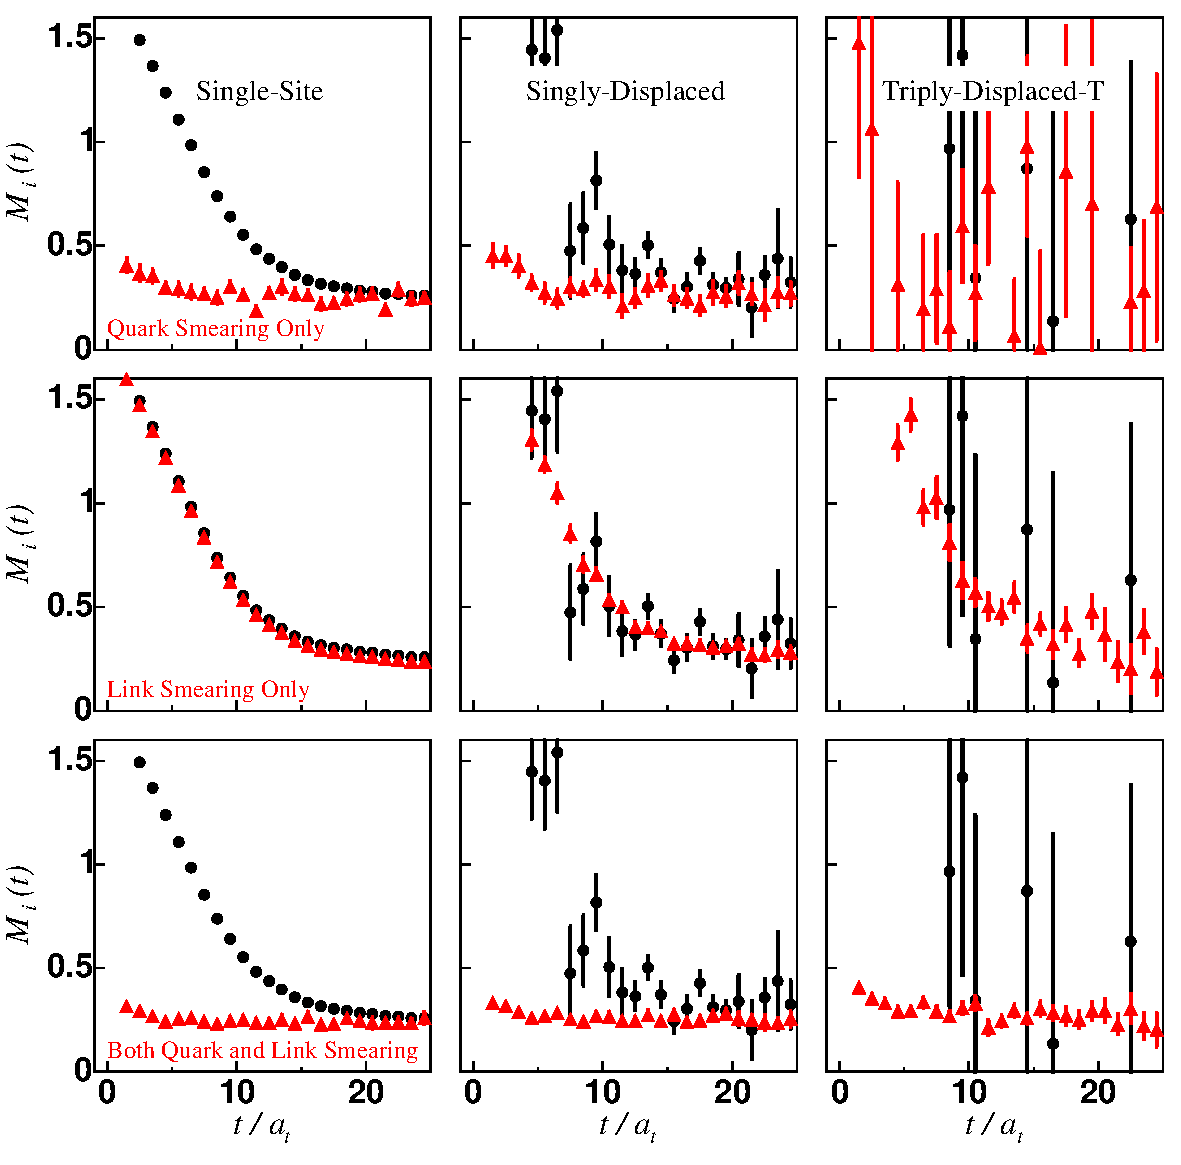
\includegraphics[scale=0.8]{figures/meff-smearing.pdf}
        \caption[Effective masses (defined in Sec.~\ref{sec:eff_mass}) $M_i(t)$ of a single nucleon for three different smearing schemes and three different displacement schemes.]{Effective masses (defined in Sec.~\ref{sec:eff_mass}) $M_i(t)$ of a single nucleon for three different smearing schemes and three different displacement schemes. Black markers denote unsmeared operators and red markers denote smeared operators. Figure taken from Ref.~\cite{spectroscopy}.}\label{fig:meff-smearing}
    \end{figure}
    
    Continuing, $\widetilde\Delta$ is Hermitian, and we denote its eigenvalues as $-\lambda^{(k)}$ (ordered by increasing $\lambda^{(k)}$) and their corresponding orthonormal eigenvectors as $v^{(k)}$. Then, if we define the smearing kernel in Eq.~(\ref{eq:quark_smearing}) as $K=\left(1+\frac{\sigma_{s}^{2}}{4 n_{\sigma}} \widetilde{\Delta}\right)^{n_{\sigma}}$, we can express the kernel in the eigenbasis of the GCL:
    \begin{equation}
        K_{a b}(x, y)=\delta_{x_{4}, y_{4}} \sum_{k} w_{k}\,v_{a}^{(k)}(x) v_{b}^{(k)}(y)^{*},
    \end{equation}
    where we suppress the flavor index, and where $w_k\in\mathbb{R}^+$. Since $K$ is written in terms of $\widetilde\Delta$, it is trivial to write down,
    \begin{equation}
        w_{k}=\left(1-\frac{\sigma_{s}^{2}}{4 n_{\sigma}} \lambda^{(k)}\right)^{n_{\sigma}}.
    \end{equation}
    It is then also easy to see that,
    \begin{equation}
        \lim _{n_{\sigma} \rightarrow \infty} w_{k}=\exp \left(-\frac{1}{4} \sigma_{s}^{2} \lambda^{(k)}\right).
    \end{equation}
    We can now see the advantage of working in the eigenbasis of the GCL: the weights, $w_{k}$, of higher modes of $\widetilde\Delta$ are exponentially suppressed. We can then investigate the possibility of modifying the weights to neglect higher-lying contributions. One simple way to accomplish this is the so-called \emph{Laplacian Heaviside} (LapH) smearing scheme, introduced by Peardon, Morningstar, et al.\ in Ref.~\cite{Peardon:2009gh}. This procedure sets the weights to be,
    \begin{equation}
        w_{k}=\Theta\left(\sigma_{s}^{2}-\lambda^{(k)}\right),
    \end{equation}
    where $\Theta$ is the Heaviside step function, and $\sigma_s^2$ acts as a hard cutoff. The LapH smearing kernel is now defined as
    \begin{equation}\label{eq:smearing_operator}
        \mathcal{S}=\Theta\left(\sigma_{s}^{2}+\widetilde{\Delta}\right),
    \end{equation}
    and our smeared quark fields are now given by
    \begin{equation}
        \widetilde\psi(x) = \mathcal{S}\psi(x).
    \end{equation}

    \subsection{Displacements}
    Hadrons are objects which are extended in space. Therefore, if we hope to capture radial and orbital structure when computing the hadronic correlation functions, then we must displace the quark fields, and do so in a gauge-covariant way. The displacements we consider are straight-path displacements along the spatial lattice unit vectors: $j = \pm 1, \pm 2, \pm 3$. We define the gauge-covariant displacement operator in the $j^{\mathrm{th}}$ direction by,
    \begin{equation}\label{eq:displacement_operator}
        \widetilde{D}_{j}^{(p)}\left(x, x^{\prime}\right)=\widetilde{U}_{j}(x) \widetilde{U}_{j}(x+\hat{j}) \ldots \widetilde{U}_{j}(x+(p-1) \hat{j}) \delta_{x^{\prime}, x+p \hat{j}},
    \end{equation}
    where $p \geq 1$ denotes the number of steps by which the field is displaced. For convenience, we also define a zero-displacement operator, $\widetilde{D}_{0}^{(p)}\left(x, x^{\prime}\right)=\delta_{x x^{\prime}}.$ Including color indices $a$ and $a^\prime$, it can be shown that $\widetilde{D}_{j}^{(p) \dagger}\left(x, x^{\prime}\right)^{a a^{\prime}}=\widetilde{D}_{-j}^{(p)}\left(x, x^{\prime}\right)^{a a^{\prime}}.$ From this, the following useful properties can be derived:
    \begin{equation}
        \begin{aligned}
            \left(\widetilde{D}_{j}^{(p)} \psi\right)(x)&=\sum_{x^{\prime}} \widetilde{D}_{j}^{(p)}\left(x, x^{\prime}\right) \psi\left(x^{\prime}\right)=\widetilde{U}_{j}(x) \widetilde{U}_{j}(x+\hat{j}) \ldots \widetilde{U}_{j}(x+(p-1) \hat{j}) \psi(x+p \hat{j}),\\
            \left(\overline{\chi} \widetilde{D}_{j}^{(p) \dagger}\right)(x)&=\sum_{x^{\prime}} \overline{\chi}\left(x^{\prime}\right) \widetilde{D}_{j}^{(p) \dagger}\left(x^{\prime}, x\right)=\sum_{x^{\prime}} \overline{\chi}\left(x^{\prime}\right) \widetilde{D}_{-j}^{(p)}\left(x^{\prime}, x\right)\\
            &=\overline{\chi}(x+p \hat{j}) \widetilde{U}_{j}^{\dagger}(x+(p-1) \hat{j}) \ldots \widetilde{U}_{j}^{\dagger}(x+\hat{j}) \widetilde{U}_{j}^{\dagger}(x),
        \end{aligned}
    \end{equation}
    from which it can be seen,
    \begin{equation}
        \overline{\chi}(x)\left(\widetilde{D}_{j}^{(p)} \psi\right)(x)=\left(\overline{\chi} \widetilde{D}_{j}^{(p)}\right)(x) \psi(x).
    \end{equation}

    The final building blocks for our hadronic operators are \emph{covariantly-displaced, smeared quark fields} and can be summarized as follows:
    \begin{equation}
        \boxed{\left(\widetilde{D}_{j_{1}}^{(p)} \ldots \widetilde{D}_{j_{n}}^{(p)} \widetilde{\psi}\right)_{a \alpha}^{A}, \quad\left(\widetilde{\chi} \widetilde{D}_{j_{1}}^{(p) \dagger} \ldots \widetilde{D}_{j_{n}}^{(p) \dagger}\right)_{a \alpha}^{A}, \quad-3 \leq j_{i} \leq 3,}
    \end{equation}
    where $A$ indexes flavor, $a$ indexes color, and $\alpha$ indexes Dirac spin.
    \section{Symmetries on the Lattice}
    Symmetries are very useful for characterizing and labeling stationary states in quantum mechanics. Conserved quantities, such as momentum and charge, emerge from the symmetries of a given system, and so in order to identify the relevant quantum numbers of a theory, we must identify its relevant symmetries. The primary symmetries we are interested in are: (cubic) rotations, $G$-parity, isospin, and flavor. SU(3) gauge symmetry is also a central component of the theory, but since all of the final objects we study are colorless, it does not contribute to how we label stationary states.
    
    \subsection{Rotations}
    Given the nature of a discrete, finite-volume lattice, one can easily see that the SO(3) rotation group is no longer a symmetry group of any lattice gauge theory. Because of this, angular momentum is not conserved on the lattice, and therefore angular momentum is no longer a good quantum number. We will see that instead of using the irreducible representations (irreps) of SO(3) to label stationary states, we use the irreps of the octahedral group.
 
    To aid in discussions of cubic rotations on the lattice, the following notation will be used, where the axes of rotation, $j = x,y,z,a,b,c,d,\alpha,\beta,\gamma,\delta$, are shown in Figure~\ref{fig:rotation_axes}:
    \begin{equation}
        \begin{aligned}
            E &: \text{the identity}\\
            C_{nj} &: \text{proper rotation of angle}\ \frac{2\pi}{n}\ \text{about the axis}\ O_j\text{, where}\ n = 2,3,4 \\
            I_s &: \text{spatial inversion}
        \end{aligned}
    \end{equation}
    \begin{figure}
        \centering
        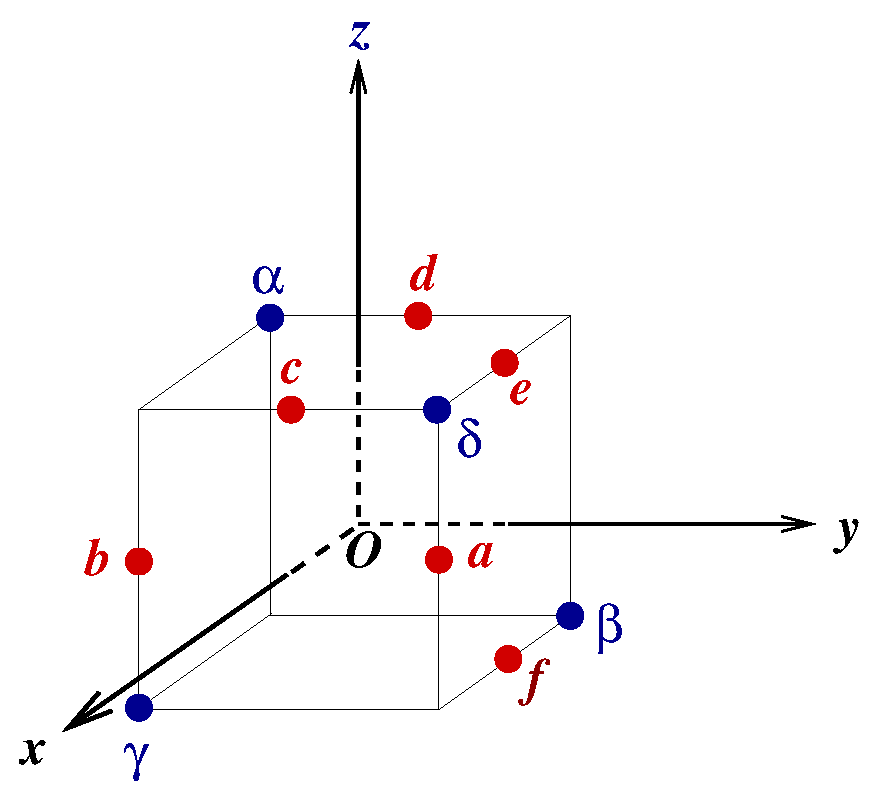
\includegraphics[scale=0.5]{figures/Oaxes.pdf}
        \caption[The rotation axes corresponding to the rotations $C_{nj}$.]{The rotation axes corresponding to the rotations $C_{nj}$. Figure taken from Ref.~\cite{spectroscopy}.}
        \label{fig:rotation_axes}
    \end{figure}
    The octahedral point group, $O$, consists of all allowed rotations on a three-dimensional spatially-isotropic cubic lattice, and contains the following elements:
    \begin{table}[h!]
        \centering
        \begin{tabular}{l|l}
            Group element & Axes, $j$\\
            \hline
            $E$ & \\
            $C_{4j}$, $C_{4j}^{-1}$ & $x,y,z$ \\
            $C_{2j}$ & $x,y,z,a,b,c,d,e,f$ \\
            $C_{3j}$, $C_{3j}^{-1}$ & $\alpha,\beta,\gamma,\delta$
        \end{tabular}
        \label{table:O}
    \end{table}

    There are five irreps of $O$. Following the Mulliken convention, they are named $A_1$, $A_2$, $E$, $T_1$, $T_2$, and they have dimensions 1, 1, 2, 3, 3, respectively. In order to make connections to infinite-volume continuum physics, the Table~\ref{table:O_occurrence_nums} gives the \emph{occurrence numbers} $n_\Gamma^J$, which are the number of times the irrep $\Gamma$ of $O$ occurs in the subduction of the irrep $J$ of SO(3).

    When we take the direct product of $O$ with the group $\lbrace E,I_s \rbrace$, adding in spatial inversions to our proper rotations, we get what is known as the point group $O_h$. This group has twice the number of irreps as $O$, and so we add the labels $g/u$ (standing for the German \emph{gerade} and \emph{ungerade}) to our irreps, which denote even and odd parity, respectively. The irreps of $O_h$ are $A_{1g}$, $A_{1u}$, $A_{2g}$, $A_{2u}$, $E_g$, $E_u$, $T_{1g}$, $T_{1u}$, $T_{2g}$, and $T_{2u}$.

    When we incorporate spin into the picture, we must introduce a new generator that represents rotating by $2\pi$ about any axis. Doing so, we arrive at the double octahedral point group $O^D$. Sparing the group-theoretical details, $O^D$ has three irreps in addition to all of the irreps of $O$. These are named $G_1$, $G_2$, and $H$, and are of dimension 2, 2, and 4, respectively. Table~\ref{table:OD_occurrence_nums} gives the occurrence numbers of these three additional irreps in the subductions of the $J$ irreps of SU(2). Like for $O_h$, when we incorporate spatial inversions into $O^D$, we arrive at the double point group $O_h^D$, which has twice the number of irreps of $O^D$. The additional irreps are $G_{1g}$, $G_{1u}$, $G_{2g}$, $G_{2u}$, $H_g$, and $H_u$.

    
    \begin{table}
        \centering
        \begin{subtable}{.49\linewidth}
        \centering
        \begin{tabular}{l|l|l|l|l|l}
            $J$ & $n_{A_1}^J$ & $n_{A_2}^J$ & $n_{E}^J$ & $n_{T_1}^J$ & $n_{T_2}^J$\\
            \hline
            0 & 1 & 0 & 0 & 0 & 0\\
            1&0&0&0&1&0\\
            2&0&0&1&0&1\\
            3&0&1&0&1&1\\
            4&1&0&1&1&1\\
            \vdots & \vdots & \vdots & \vdots & \vdots & \vdots
        \end{tabular}
        \caption{}
        \label{table:O_occurrence_nums}
        \end{subtable}
        \begin{subtable}{.49\linewidth}
        \centering
        \begin{tabular}{l|l|l|l}
            $J$ & $n_{G_1}^J$ & $n_{G_2}^J$ & $n_{H}^J$ \\
            \hline
            $\frac{1}{2}$&1&0&0\\
            $\frac{3}{2}$&0&0&1\\
            $\frac{5}{2}$&0&1&1\\
            $\frac{7}{2}$&1&1&1\\
            $\frac{9}{2}$&1&0&2\\
            \vdots&\vdots&\vdots&\vdots
        \end{tabular}
        \caption{}
        \label{table:OD_occurrence_nums}
        \end{subtable}
        \caption{Occurrence numbers for (a) integer values of angular momentum and (b) half-integer values of angular momentum}
    \end{table}
    
    \subsubsection{Moving irreps}
    In order to identify operators that create and annihilate particles of definite momentum $\boldsymbol p$, we must subduce the representations of $O_h^D$ onto the little group of $\boldsymbol p$. The little group of $\boldsymbol p$ consists of the subgroup of the abelian group of lattice transformations which leave the momentum invariant. For $\boldsymbol p = (0, 0, 0)$, the little group is simply the point group $O_h$. For any on-axis momentum, e.g.\ $\boldsymbol p = (0, 0, 1)$, the little group is $C_{4v}$, which includes four rotations of angle $\frac{\pi}{2}$ about the axis along $\boldsymbol p$, as well as four reflections about reflection planes containing that axis. The group elements are contained in three conjugacy classes, which are given in Table~\ref{table:C4v}.  For any planar-diagonal momentum, e.g.\ $\boldsymbol p = (0, 1, 1)$, the little group is $C_{2v}$, the elements and conjugacy classes of which are given in Table~\ref{table:C2v}. For any cubic-diagonal momentum, e.g.\ $\boldsymbol p = (1,1,1)$, the little group is $C_{3v}$; its elements and their conjugacy classes are given in Table~\ref{table:C3v}. Additionally, in order to construct the analogous spinorial little groups (called $C_{4v}^D$, $C_{2v}^D$, and $C_{3v}^D$, respectively), we include the $2\pi$-rotation generator $\overline E$. Tables~\ref{table:C4vD}---\ref{table:C3vD} give the elements and conjugacy classes for the spinorial little groups.
    
    % \begin{table}
    %     \begin{minipage}[t]{0.32\linewidth}
    %         \centering
    %         \begin{tabular}[t]{|l|l|}
    %             \hline
    %             $C_{4v}$ & \\
    %             \hline
    %             $\mathcal{C}_{1}$ & $\{E\}$ \\
    %             $\mathcal{C}_{2}$ & $\{C_{2 z}\}$ \\
    %             $\mathcal{C}_{3}$ & $\{C_{4 z}, C_{4 z}^{-1}\}$ \\
    %             $\mathcal{C}_{4}$ & $\{I_{s} C_{2 x}, I_{s} C_{2 y}\}$ \\
    %             $\mathcal{C}_{5}$ & $\{I_{s} C_{2 a}, I_{s} C_{2 b}\}$ \\
    %             \hline
    %         \end{tabular}
    %         \caption{Group elements and conjugacy classes for the little group $C_{4v}$.}
    %         \label{table:C4v}
    %     \end{minipage}
    %     \begin{minipage}[t]{0.32\linewidth}
    %         \centering
    %         \begin{tabular}[t]{|l|l|}
    %             \hline
    %             $C_{2v}$ & \\
    %             \hline
    %             $\mathcal{C}_{1}$ & $\{E\}$ \\
    %             $\mathcal{C}_{2}$ & $\{C_{2 e}\}$ \\
    %             $\mathcal{C}_{3}$ & $\{I_{s} C_{2 f}\}$ \\
    %             $\mathcal{C}_{4}$ & $\{I_{s} C_{2 x}\}$ \\
    %             \hline
    %             \multicolumn{2}{}{}
    %         \end{tabular}
    %         \caption{Group elements and conjugacy classes for the little group $C_{2v}$.}
    %         \label{table:C2v}
    %     \end{minipage}
    %     \begin{minipage}[t]{0.32\linewidth}
    %         \centering
    %         \begin{tabular}[t]{|l|l|}
    %             \hline
    %             $C_{3v}$ & \\
    %             \hline
    %             $\mathcal{C}_{1}$ & $\{E\}$ \\
    %             $\mathcal{C}_{2}$ & $\{C_{3 \delta}, C_{3 \delta}^{-1}\}$ \\
    %             $\mathcal{C}_{3}$ & $\{I_{s} C_{2 b}, I_{s} C_{2 d}, I_{s} C_{2 f}\}$\\
    %             \hline
    %             \multicolumn{2}{}{}\\
    %             \multicolumn{2}{}{}
    %         \end{tabular}
    %         \caption{Group elements and conjugacy classes for the little group $C_{3v}$.}
    %         \label{table:C3v}
    %     \end{minipage}
    % \end{table}               
    % \begin{table}
    %     \begin{minipage}[t]{0.32\linewidth}
    %         \centering
    %         \begin{tabular}[t]{|l|l|}
    %             \hline
    %             $C_{4vD}$ & \\
    %             \hline
    %             $\mathcal{C}_{1}$ & $\{E\}$ \\
    %             $\mathcal{C}_{2}$ & $\{C_{2 z}, \overline{C}_{2 z}\}$ \\
    %             $\mathcal{C}_{3}$ & $\{C_{4 z}, C_{4 z}^{-1}\}$ \\
    %             $\mathcal{C}_{4}$ & $\{I_{s} C_{2 x}, I_{s} C_{2 y},$\\
    %             & $\quad I_{s} \overline{C}_{2 x}, I_{s} \overline{C}_{2 y}\}$ \\
    %             $\mathcal{C}_{5}$ & $\{I_{s} C_{2 a}, I_{s} C_{2 b},$\\
    %             & $\quad I_{s} \overline{C}_{2 a}, I_{s} \overline{C}_{2 b}\}$ \\
    %             $\mathcal{C}_{6}$ & $\{\overline{E}\}$ \\
    %             $\mathcal{C}_{7}$ & $\{\overline{C}_{4 z}, \overline{C}_{4 z}^{-1}\}$\\
    %             \hline
    %         \end{tabular}
    %         \caption{Group elements and conjugacy classes for the little group $C_{4v}^D$.}
    %         \label{table:C4vD}
    %     \end{minipage}
    %     \begin{minipage}[t]{0.32\linewidth}
    %         \centering
    %         \begin{tabular}[t]{|l|l|}
    %             \hline
    %             $C_{2vD}$ & \\
    %             \hline
    %             $\mathcal{C}_{1}$ & $\{E\}$ \\
    %             $\mathcal{C}_{2}$ & $\{C_{2 e}, \overline{C}_{2 e}\}$ \\
    %             $\mathcal{C}_{3}$ & $\{I_{s} C_{2 f}, I_{s} \overline{C}_{2 f}\}$ \\
    %             $\mathcal{C}_{4}$ & $\{I_{s} C_{2 x}, I_{s} \overline{C}_{2  x}\}$ \\
    %             $\mathcal{C}_{5}$ & $\{\overline{E}\}$\\
    %             \hline
    %             \multicolumn{2}{}{}\\
    %             \multicolumn{2}{}{}\\
    %             \multicolumn{2}{}{}\\
    %             \multicolumn{2}{}{}
    %         \end{tabular}
    %         \caption{Group elements and conjugacy classes for the little group $C_{2v}^D$.}
    %         \label{table:C2vD}
    %     \end{minipage}
    %     \begin{minipage}[t]{0.32\linewidth}
    %         \centering
    %         \begin{tabular}[t]{|l|l|}
    %             \hline
    %             $C_{3vD}$ & \\
    %             \hline
    %             $\mathcal{C}_{1}$ & $\{E\}$ \\
    %             $\mathcal{C}_{2}$ & $\{C_{3 \delta}, C_{3 \delta}^{-1}\}$ \\
    %             $\mathcal{C}_{3}$ & $\{I_{s} C_{2 b}, I_{s} C_{2 d}, I_{s} C_{2 f}\}$ \\
    %             $\mathcal{C}_{4}$ & $\{\overline{E}\}$ \\
    %             $\mathcal{C}_{5}$ & $\{\overline{C}_{3 \delta}, \overline{C}_{3 \delta}^{-1}\}$ \\
    %             $\mathcal{C}_{6}$ & $\{I_{s} \overline{C}_{2 b}, I_{s} \overline{C}_{2 d}, I_{s} \overline{C}_{2 f}\}$\\
    %             \hline
    %             \multicolumn{2}{}{}\\
    %             \multicolumn{2}{}{}\\
    %             \multicolumn{2}{}{}
    %         \end{tabular}
    %         \caption{Group elements and conjugacy classes for the little group $C_{3v}^D$.}
    %         \label{table:C3vD}
    %     \end{minipage}
    % \end{table}               
    \begin{table}
        \begin{subtable}[t]{0.32\linewidth}
            \centering
            \begin{tabular}[t]{|l|l|}
                \hline
                $C_{4v}$ & \\
                \hline
                $\mathcal{C}_{1}$ & $\{E\}$ \\
                $\mathcal{C}_{2}$ & $\{C_{2 z}\}$ \\
                $\mathcal{C}_{3}$ & $\{C_{4 z}, C_{4 z}^{-1}\}$ \\
                $\mathcal{C}_{4}$ & $\{I_{s} C_{2 x}, I_{s} C_{2 y}\}$ \\
                $\mathcal{C}_{5}$ & $\{I_{s} C_{2 a}, I_{s} C_{2 b}\}$ \\
                \hline
            \end{tabular}
            \caption{}
            \label{table:C4v}
        \end{subtable}
        \begin{subtable}[t]{0.32\linewidth}
            \centering
            \begin{tabular}[t]{|l|l|}
                \hline
                $C_{2v}$ & \\
                \hline
                $\mathcal{C}_{1}$ & $\{E\}$ \\
                $\mathcal{C}_{2}$ & $\{C_{2 e}\}$ \\
                $\mathcal{C}_{3}$ & $\{I_{s} C_{2 f}\}$ \\
                $\mathcal{C}_{4}$ & $\{I_{s} C_{2 x}\}$ \\
                \hline
                % \multicolumn{2}{}{}
            \end{tabular}
            \caption{}
            \label{table:C2v}
        \end{subtable}
        \begin{subtable}[t]{0.32\linewidth}
            \centering
            \begin{tabular}[t]{|l|l|}
                \hline
                $C_{3v}$ & \\
                \hline
                $\mathcal{C}_{1}$ & $\{E\}$ \\
                $\mathcal{C}_{2}$ & $\{C_{3 \delta}, C_{3 \delta}^{-1}\}$ \\
                $\mathcal{C}_{3}$ & $\{I_{s} C_{2 b}, I_{s} C_{2 d}, I_{s} C_{2 f}\}$\\
                \hline
                % \multicolumn{2}{}{}\\
                % \multicolumn{2}{}{}
            \end{tabular}
            \caption{}
            \label{table:C3v}
        \end{subtable}\\\\
        \begin{subtable}[t]{0.32\linewidth}
            \centering
            \begin{tabular}[t]{|l|l|}
                \hline
                $C_{4vD}$ & \\
                \hline
                $\mathcal{C}_{1}$ & $\{E\}$ \\
                $\mathcal{C}_{2}$ & $\{C_{2 z}, \overline{C}_{2 z}\}$ \\
                $\mathcal{C}_{3}$ & $\{C_{4 z}, C_{4 z}^{-1}\}$ \\
                $\mathcal{C}_{4}$ & $\{I_{s} C_{2 x}, I_{s} C_{2 y},$\\
                & $\quad I_{s} \overline{C}_{2 x}, I_{s} \overline{C}_{2 y}\}$ \\
                $\mathcal{C}_{5}$ & $\{I_{s} C_{2 a}, I_{s} C_{2 b},$\\
                & $\quad I_{s} \overline{C}_{2 a}, I_{s} \overline{C}_{2 b}\}$ \\
                $\mathcal{C}_{6}$ & $\{\overline{E}\}$ \\
                $\mathcal{C}_{7}$ & $\{\overline{C}_{4 z}, \overline{C}_{4 z}^{-1}\}$\\
                \hline
            \end{tabular}
            \caption{}
            \label{table:C4vD}
        \end{subtable}
        \begin{subtable}[t]{0.32\linewidth}
            \centering
            \begin{tabular}[t]{|l|l|}
                \hline
                $C_{2vD}$ & \\
                \hline
                $\mathcal{C}_{1}$ & $\{E\}$ \\
                $\mathcal{C}_{2}$ & $\{C_{2 e}, \overline{C}_{2 e}\}$ \\
                $\mathcal{C}_{3}$ & $\{I_{s} C_{2 f}, I_{s} \overline{C}_{2 f}\}$ \\
                $\mathcal{C}_{4}$ & $\{I_{s} C_{2 x}, I_{s} \overline{C}_{2  x}\}$ \\
                $\mathcal{C}_{5}$ & $\{\overline{E}\}$\\
                \hline
                % \multicolumn{2}{}{}\\
                % \multicolumn{2}{}{}\\
                % \multicolumn{2}{}{}\\
                % \multicolumn{2}{}{}
            \end{tabular}
            \caption{}
            \label{table:C2vD}
        \end{subtable}
        \begin{subtable}[t]{0.32\linewidth}
            \centering
            \begin{tabular}[t]{|l|l|}
                \hline
                $C_{3vD}$ & \\
                \hline
                $\mathcal{C}_{1}$ & $\{E\}$ \\
                $\mathcal{C}_{2}$ & $\{C_{3 \delta}, C_{3 \delta}^{-1}\}$ \\
                $\mathcal{C}_{3}$ & $\{I_{s} C_{2 b}, I_{s} C_{2 d}, I_{s} C_{2 f}\}$ \\
                $\mathcal{C}_{4}$ & $\{\overline{E}\}$ \\
                $\mathcal{C}_{5}$ & $\{\overline{C}_{3 \delta}, \overline{C}_{3 \delta}^{-1}\}$ \\
                $\mathcal{C}_{6}$ & $\{I_{s} \overline{C}_{2 b}, I_{s} \overline{C}_{2 d}, I_{s} \overline{C}_{2 f}\}$\\
                \hline
                % \multicolumn{2}{}{}\\
                % \multicolumn{2}{}{}\\
                % \multicolumn{2}{}{}
            \end{tabular}
            \caption{}
            \label{table:C3vD}
        \end{subtable}
        \caption{Group elements and conjugacy classes for the momentum little groups.}
    \end{table}
    Finally, the subductions of the irreps of $O_h^D$ onto the above little groups leaves us with the irreps in which we expect to find moving particles. These subductions are given in Table~\ref{table:subductions}.
    \begin{table}
        \centering
        \begin{tabular}{c|c|c|c}
            $\Lambda(O_h)$ & $\Lambda(O_h)\downarrow C_{4v}$ & $\Lambda(O_h) \downarrow C_
            {3v}$ & $\Lambda(O_h) \downarrow C_{2v}$ \\
            \hline
            $A_{1g}$ & $A_1$ & $A_1$ & $A_1$ \\
            $A_{1u}$ & $A_2$ & $A_2$ & $A_2$ \\
            $A_{2g}$ & $B_1$ & $A_2$ & $B_2$ \\
            $A_{2u}$ & $B_2$ & $A_1$ & $B_1$ \\
            $E_g$ & $A_1 \oplus B_1$ & $E$ & $A_1 \oplus B_2$ \\
            $E_u$ & $A_2 \oplus B_2$ & $E$ & $A_2 \oplus B_1$ \\
            $T_{1g}$ & $A_2 \oplus E$ & $A_2 \oplus E$ & $A_2 \oplus B_1 \oplus B_2$ \\
            $T_{1u}$ & $A_1 \oplus E$ & $A_1 \oplus E$ & $A_1 \oplus B_1 \oplus B_2$ \\
            $T_{2g}$ & $B_2 \oplus E$ & $A_1 \oplus E$ & $A_1 \oplus A_2 \oplus B_1$ \\
            $T_{2u}$ & $B_1 \oplus E$ & $A_2 \oplus E$ & $A_1 \oplus A_2 \oplus B_2$ \\
            $G_{1g/u}$ & $G_1$ & $G$ & $G$ \\
            $G_{2g/u}$ & $G_2$ & $G$ & $G$ \\
            $H_{g/u}$ & $G_1 \oplus G_2$ & $F_1 \oplus F_2 \oplus G$ & $2G$
        \end{tabular}
        \caption{Subductions of the irreps of the octahedral group onto the irreps of the little groups $C_{4v}$, $C_{3v}$, and $C_{2v}$.}
        \label{table:subductions}
    \end{table}
    
    \subsection{Isospin and Quark Flavor}
    In the $\overline{\rm{MS}}$ renormalization scheme at a scale of $\sim 2$ GeV, the so-called ``current-quark mass'' of the up quark is $m_u = 2.16^{+0.49}_{-0.26}$ MeV and that of the down quark is $m_d = 4.67^{+0.48}_{-0.17}$ MeV~\cite{PhysRevD.98.030001}. While these masses differ by more than a factor of 2, their difference is very small compared to the next heaviest quark, which is the strange quark, measuring at $m_s = 93^{+11}_{-5}$ MeV~\cite{PhysRevD.98.030001}. Therefore, we find it justified to make an approximation and set $m_u = m_d$ in our calculations. Since pure QCD also conserves flavor (we do not include electroweak interactions), our theory now possesses an internal SU(2) symmetry, the conserved quantity of which is referred to as \emph{isospin}. This has the same mathematical structure as normal spin, and we can therefore think of it analogously, but it should be stressed that isospin has no relation to physical space and does not denote any kind of angular momentum. The up quark and down quark states can then be thought of as a doublet of states having total isospin $I=\frac{1}{2}$. Just like with SU(2) spin, isospin can be decomposed onto three axes. By convention, we assign the third isospin axis component of the up quark to be $I_3 = \frac{1}{2}$ and of the down quark to be $I_3 = -\frac{1}{2}$. Their corresponding antiparticles have the same $I$, but $I_3\rightarrow -I_3$. The work presented here is done in a theory of $N_f = 2 + 1$ QCD, meaning our theory contains two \emph{light} quarks, referring to the up and down quarks, and a strange quark. (The strange quark is sometimes referred to as a light quark in other contexts, such as in Ref.~\cite{PhysRevD.98.030001}.)
    
    Under an SU(2) isospin rotation of the form
    \begin{equation}
        U_{R_{\tau}}=\exp{-i\alpha\tau_3}\exp{-i\beta\tau_2}\exp{-i\gamma\tau_3} = \exp (-i \boldsymbol{\varphi} \cdot \boldsymbol{\tau}),
    \end{equation}
    where $\tau_1$, $\tau_2$, $\tau_3$ are the three generators of isospin rotations,
    an operator $\overline O_{I_3}^{(I)}$ transforms according to the $I$ irreducible representation as
    \begin{equation}
        U_{R_{\tau}}\overline O_{I_3}^{(I)}U_{R_{\tau}}^\dagger = \sum_{I_3^\prime} \overline O_{I_3^\prime}^{(I)} D^{(I)}_{I_3^\prime, I_3}(R_\tau),
    \end{equation}
    where $D^{(I)}(R_\tau)$ are the Wigner rotation matrices. In order for an operator $\overline O_{I_3}^{(I)}$ to transform irreducibly under isospin, it must satisfy the following properties:
    \begin{align}
        \left[\tau_3, \overline O_{I_3}^{(I)}\right] &= I_3 \overline O_{I_3}^{(I)}, \\
        \left[\tau_+, \overline O_{I_3}^{(I)}\right] &= \sqrt{(I - I_3)(I + I_3 + 1)} \overline O_{I_3 + 1}^{(I)}, \\
        \left[\tau_-, \overline O_{I_3}^{(I)}\right] &= \sqrt{(I + I_3)(I - I_3 + 1)} \overline O_{I_3 - 1}^{(I)}, \\
        \left[\tau_3, \left[\tau_3, \overline O_{I_3}^{(I)}\right] \right] + \frac{1}{2} \left[\tau_+, \left[\tau_-, \overline O_{I_3}^{(I)}\right]\right] &+ \frac{1}{2}\left[\tau_-, \left[\tau_+, \overline O_{I_3}^{(I)}\right]\right] = I(I + 1) \overline O_{I_3}^{(I)},
    \end{align}
    where $\tau_\pm = \tau_1 \pm i\tau_2$. For annihilation operators, an operator $O_{I_3}^{(I)}$ should transform according to the $I$ irreducible representation as
    \begin{equation}
        U_{R_{\tau}}O_{I_3}^{(I)}U_{R_{\tau}}^\dagger = \sum_{I_3^\prime} O_{I_3^\prime}^{(I)} D^{(I)}_{I_3^\prime, I_3}(R_\tau)^*.
    \end{equation}
    Annihilation operators that are irreducible under isospin rotations should satisfy:
    \begin{align}
        \left[\tau_3, O_{I_3}^{(I)}\right] &= -I_3 O_{I_3}^{(I)}, \\
        \left[\tau_+, O_{I_3}^{(I)}\right] &= -\sqrt{(I - I_3)(I + I_3 + 1)} O_{I_3 + 1}^{(I)}, \\
        \left[\tau_-, O_{I_3}^{(I)}\right] &= -\sqrt{(I + I_3)(I - I_3 + 1)} O_{I_3 - 1}^{(I)}, \\
        \left[\tau_3, \left[\tau_3, O_{I_3}^{(I)}\right] \right] + \frac{1}{2} \left[\tau_+, \left[\tau_-, O_{I_3}^{(I)}\right]\right] &+ \frac{1}{2}\left[\tau_-, \left[\tau_+, O_{I_3}^{(I)}\right]\right] = I(I + 1)  O_{I_3}^{(I)}.
    \end{align}
    \subsection{Charge Conjugation and $G$-Parity}
    $C$-parity can only be a symmetry for electrically neutral states, but as electric charge is not a relevant quantity in pure QCD, we are motivated to generalize $C$-parity in order to account states in a charged isospin multiplet, such as the pion triplet. With $\mathcal C$ denoting the charge conjugation operator, $G$-parity can be explicitly defined as
    \begin{equation}
        U_G = \mathcal C e^{-i\pi\tau_2}.
    \end{equation}
    Since charge conjugation is a symmetry of the strong interaction, then when isospin is also a symmetry, $G$-parity must be a symmetry as well. The basic building blocks transform under $G$-parity as follows. Here, $\Gamma^G$ is the representation matrix for $U_G$ and is equal to $\gamma_2$ in the Dirac-Pauli, Weyl, and DeGrand-Rossi conventions.
    \begin{align} U_{G}\left(D_{j} \mathcal S \psi(x)\right)_{a \alpha}^{u} U_{G}^{\dagger} &=-\left(\chi \mathcal S D_{j}^{\dagger}(x)\right)_{a \beta}^{d} \Gamma_{\beta \alpha}^{G}, \\ U_{G}\left(D_{j}\mathcal S \psi(x)\right)_{a \alpha}^{d} U_{G}^{\dagger} &=\left(\chi \mathcal S D_{j}^{\dagger}(x)\right)_{a \beta}^{u} \Gamma_{\beta \alpha}^{G}, \\ U_{G}\left(D_{j} \mathcal S \psi(x)\right)_{a \alpha}^{s} U_{G}^{\dagger} &=-\left(\chi \mathcal S D_{j}^{\dagger}(x)\right)_{a \beta}^{s} \Gamma_{\beta \alpha}^{G}, \\ U_{G}\left(\chi \mathcal S D_{j}^{\dagger}(x)\right)_{a \alpha}^{u} U_{G}^{\dagger} &=-\Gamma_{\alpha \beta}^{C}\left(D_{j} \mathcal S \psi(x)\right)_{a \beta}^{u}, \\ U_{G}\left(\chi \mathcal S D_{j}^{\dagger}(x)\right)_{a \alpha}^{a} U_{G}^{\dagger} &=\Gamma_{\alpha \beta}^{G}\left(D_{j} \mathcal S \psi(x)\right)_{a \beta^{\prime}}^{u}, \\ U_{G}\left(\chi \mathcal S D_{j}^{\dagger}(x)\right)_{a \alpha}^{s} U_{G}^{\dagger} &=-\Gamma_{\alpha \beta}^{C}\left(D_{j} \mathcal S \psi(x)\right)_{a \beta}^{s}. \end{align}
    \section{Single-Hadron Operator Construction}
    States in continuum, $N_f=2+1$, pure QCD are classified according to: momentum $\boldsymbol p$, total spin $J$, spin projection $J_z$ (or any other axis), parity $P = \pm 1$ (at rest), isospin, strangeness, and $G$-parity (for hadron multiplets with an average electric charge of zero). In order to construct single-hadron operators, we first start with \emph{elemental} single-hadron operators. An elemental operator is simply one that is constructed with proper color structure (i.e.\ it is gauge-invariant), definite flavor structure, definite position or momentum, but has not been projected onto relevant symmetry sectors.
    \subsection{Elemental Single-Hadron Operators}
    \subsubsection{Elemental Baryon Operators}
    An elemental baryon operator can be denoted by $\Phi_{\alpha \beta \gamma; ijk}^{ABC}(\bs p, t)$. Capital Latin indices denote flavor, Greek indices denote Dirac spin, and lowercase Latin indices denote displacement type (to be defined shortly). $\bs p$ and $t$ denote momentum and time slice. Note that there are no indices for color, since the final operators must be colorless. In order to ensure proper color structure (i.e.\ in order to construct gauge invariant operators), there is only one way to do so, which is by use of the Levi-Civita coupling $\varepsilon_{abc}$. In order to construct a single-site (i.e.\ no displacement) three-quark object out of three smeared and displaced quark fields, we form their product with a Levi-Civita coupling:
    \begin{equation}
       \varepsilon_{a b c} \widetilde{\psi}_{a \alpha}^{A} \widetilde{\psi}_{b \beta}^{B} \widetilde{\psi}_{c \gamma}^{C}.
    \end{equation}
    To see that this is invariant under an SU(3) transformation $\widetilde\psi_a \rightarrow U_{a a^\prime} \widetilde\psi_{a^\prime}$, we use the fact that $\det[U] = 1$:
    \begin{equation}
        \begin{aligned}
            \varepsilon_{a b c} \widetilde{\psi}_{a \alpha}^{A} \widetilde{\psi}_{b \beta}^{B} \widetilde{\psi}_{c \gamma}^{C} &\rightarrow \varepsilon_{abc} U_{a a^\prime} \widetilde{\psi}_{a^\prime \alpha}^A U_{b b^\prime} \widetilde{\psi}_{b^\prime \beta}^B U_{c c^\prime} \widetilde{\psi}_{c^\prime \gamma}^C \\
            & = \det[U]\varepsilon_{a^\prime b^\prime c^\prime} \widetilde{\psi}_{a^\prime \alpha}^{A} \widetilde{\psi}_{b^\prime \beta}^{B} \widetilde{\psi}_{c^\prime \gamma}^{C} \\
            & = \varepsilon_{a b c} \widetilde{\psi}_{a \alpha}^{A} \widetilde{\psi}_{b \beta}^{B} \widetilde{\psi}_{c \gamma}^{C}
        \end{aligned}
    \end{equation}
    We do not restrict ourselves to single-site operators, however. We consider \mbox{singly-,} \mbox{doubly-,} and triply-displaced operators. For convenience, all configurations for displaced baryon operators are shown in Figure~\ref{fig:baryon_displacements}. For simplicity, we choose to displace each quark field in each single-hadron-operator by the same length $p$. A singly-displaced operator can be written as
    \begin{equation}
        \varepsilon_{a b c} \widetilde{\psi}_{a \alpha}^{A} \widetilde{\psi}_{b \beta}^{B}\left(\widetilde{D}_{j}^{(p)} \widetilde{\psi}\right)_{c \gamma}^{C}.
    \end{equation}
    A doubly-displaced operator has two configurations, an ``I'' configuration and an ``L'' configuration. A doubly-displaced-I operator is given by
    \begin{equation}
        \varepsilon_{a b c} \widetilde{\psi}_{a \alpha}^{A}\left(\widetilde{D}_{-j}^{(p)} \widetilde{\psi}\right)_{b \beta}^{B}\left(\widetilde{D}_{j}^{(p)} \widetilde{\psi}\right)_{c \gamma}^{C},
    \end{equation}
    a doubly-displaced-L operator is given by
    \begin{equation}
        \varepsilon_{a b c} \widetilde{\psi}_{a \alpha}^{A}\left(\widetilde{D}_{j}^{(p)} \widetilde{\psi}\right)_{b \beta}^{B}\left(\widetilde{D}_{k}^{(p)} \widetilde{\psi}\right)_{c \gamma}^{C} \qquad |j| \neq |k|,
    \end{equation}
    a triply-displaced-T operator is given by
    \begin{equation}
        \varepsilon_{a b c}\left(\widetilde{D}_{-j}^{(p)} \widetilde{\psi}\right)_{a \alpha}^{A}\left(\widetilde{D}_{j}^{(p)} \widetilde{\psi}\right)_{b \beta}^{B}\left(\widetilde{D}_{k}^{(p)} \widetilde{\psi}\right)_{c \gamma}^{C} \qquad |j| \neq |k|,
    \end{equation}
    and finally, a triply-displaced-O operator is given by
    \begin{equation}
        \varepsilon_{a b c}\left(\widetilde{D}_{i}^{(p)} \widetilde{\psi}\right)_{a \alpha}^{A}\left(\widetilde{D}_{j}^{(p)} \widetilde{\psi}\right)_{b \beta}^{B}\left(\widetilde{D}_{k}^{(p)} \widetilde{\psi}\right)_{c \gamma}^{C} \qquad |i| \neq |j| \neq |k|.
    \end{equation}
    We can then write down the final expression for an elemental baryon and an elemental antibaryon operator, projected onto definite momentum $\bs p$:
    \begin{equation}
        \begin{aligned}
        \Phi_{\alpha \beta \gamma ; i j k}^{A B C}(\bs p, t) &= \sum_{\boldsymbol{x}} e^{-i\bs p \cdot \bs x}\, \varepsilon_{a b c}\left(\widetilde{D}_{i}^{(p)} \widetilde{\psi}\right)_{a \alpha}^{A}(\boldsymbol{x}, t)\left(\widetilde{D}_{j}^{(p)} \widetilde{\psi}\right)_{b \beta}^{B}(\boldsymbol{x}, t)\left(\widetilde{D}_{k}^{(p)} \widetilde{\psi}\right)_{c \gamma}^{C}(\boldsymbol{x}, t) \\
        \overline\Phi_{\alpha \beta \gamma ; i j k}^{A B C}(\bs p, t) &= \sum_{\boldsymbol{x}} e^{i\bs p \cdot \bs x}\, \varepsilon_{a b c}\left(\widetilde{\chi} \widetilde{D}_{k}^{(p)\dagger} \right)_{c \gamma}^{C}(\boldsymbol{x}, t)\left(\widetilde{\chi}\widetilde{D}_{j}^{(p)\dagger}\right)_{b \beta}^{B}(\boldsymbol{x}, t)\left(\widetilde{\chi}\widetilde{D}_{i}^{(p)\dagger}\right)_{a \alpha}^{A}(\boldsymbol{x}, t),
        \end{aligned}
    \end{equation}
    where we sum over all spatial lattice sites $\bs x$ to project onto definite momentum.
    \begin{figure}
          \begin{center}
            \begin{tabular}{c c c}
              {\setlength{\unitlength}{1mm}
                \thicklines
                \begin{picture}(6,6)
                    \put(3,1.5){\circle{6}}
                    \put(2,1){\circle*{2}}
                    \put(4,1){\circle*{2}}
                    \put(3,3){\circle*{2}}
              \end{picture}} &
              {\setlength{\unitlength}{1mm}
                \thicklines
                \begin{picture}(10,4)
                    \put(0,2.2){\circle{5}}
                    \put(0,1){\circle*{2}}
                    \put(0,3.3){\circle*{2}}
                    \put(10,2){\circle*{2}}
                    \put(2.5,2){\line(1,0){7}}
              \end{picture}} &
              {\setlength{\unitlength}{1mm}
                \thicklines
                \begin{picture}(20,6)
                \put(10,3){\circle{3}}
                \put(10,3){\circle*{2}}
                \put(0,3){\circle*{2}}
                \put(20,3){\circle*{2}}
                \put(0,3){\line(1,0){8.2}}
                \put(20,3){\line(-1,0){8.2}}
                \end{picture}} \\ [4pt]
                single-site & singly-displaced & doubly-displaced-I \\ \\ \\ \\
              {\setlength{\unitlength}{1mm}
                \thicklines
                \begin{picture}(10,10)
                \put(0,0){\circle{3}}
                \put(0,0){\circle*{2}}
                \put(0,10){\circle*{2}}
                \put(10,0){\circle*{2}}
                \put(10,0){\line(-1,0){8.2}}
                \put(0,10){\line(0,-1){8.2}}
                \end{picture}} &
                {\setlength{\unitlength}{1mm}
                \thicklines
                \begin{picture}(20,10)
                \put(10,10){\circle{2}}
                \put(0,10){\circle*{2}}
                \put(20,10){\circle*{2}}
                \put(10,0){\circle*{2}}
                \put(0,10){\line(1,0){9}}
                \put(20,10){\line(-1,0){9}}
                \put(10,0){\line(0,1){9}}
                \end{picture}} &
                {\setlength{\unitlength}{1mm}
                \thicklines
                \begin{picture}(20,10)
                \put(10,10){\circle{2}}
                \put(4,2){\circle*{2}}
                \put(20,10){\circle*{2}}
                \put(10,0){\circle*{2}}
                \put(4,2){\line(3,4){5.5}}
                \put(20,10){\line(-1,0){9}}
                \put(10,0){\line(0,1){9}}
                \end{picture}}
              \\[4pt]
               doubly-displaced-L &
              triply-displaced-T & triply-displaced-O
            \end{tabular}
          \end{center}
          \caption[Diagrammatic depiction of baryon displacements.]{Diagrammatic depiction of baryon displacements, taken from Ref.~\cite{Basak:2005aq}.}
          \label{fig:baryon_displacements}
      \end{figure}

    Categorizing baryon flavor proceeds as follows. In $N_f=2+1$ QCD, our baryons can have possible total isospin values of $I=0, \frac{1}{2}, 1, \frac{3}{2}$, with $-I \leq I_3 \leq I$. A strange quark is said to have strangeness $S=-1$, and so our baryons can possess strangeness values of $S=0, -1, -2, -3$. (Antibaryons can have corresponding positive values of $S$). Table~\ref{table:baryon_names} gives the possible quark combinations, their isospin and strangeness values, and their baryon names. The different SU(2) flavor combinations are given in Table~\ref{table:baryon_flavor}. The final flavor structures of the maximal-$I_3$ elemental baryon operators are given in Table~\ref{table:hadron_flavor_structure}.
    
    \begin{table}
        \centering
        \begin{tabular}{c|cc|l}
            Quarks & $I$           & $S$ & Baryon Names\\
            \hline
            $lll$    & $\frac{1}{2}$ &  0  & $n$, $p$\\
            $lll$    & $\frac{3}{2}$ &  0  & $\Delta^-$, $\Delta^0$, $\Delta^+$, $\Delta^{++}$\\
            $lls$    & 0             & -1  & $\Lambda^0$\\
            $lls$    & 1             & -1  & $\Sigma^-$, $\Sigma^0$, $\Sigma^+$\\
            $lss$    & $\frac{1}{2}$ & -2  & $\Xi^-$, $\Xi^0$\\
            $sss$    & 0             & -3  & $\Omega^-$
        \end{tabular}
        \caption{Quark content for different baryons. ($l$ refers to \emph{light} quark, i.e.\ $u$ or $d$.)}
        \label{table:baryon_names}
    \end{table}
    \begin{table}
        \centering
        \begin{minipage}{.49\linewidth}
            \centering
            \begin{tabular}{|c|c|c|l|}
                \hline
                $I$ & $I_3$ & $S$ & SU(2) flavor \\
                \hline
                $\half$ & $\half$ & 0 & $\sqrt{\half}(\ket{udu} - \ket{duu})$ \\
                $\half$ & $\half$ & 0 & $\sqrt{\frac{1}{6}}(2\ket{uud} - \ket{udu} - \ket{duu})$ \\
                $\half$ & $-\half$ & 0 & $\sqrt{\half}(\ket{udd} - \ket{dud})$ \\
                $\half$ & $-\half$ & 0 & $\sqrt{\frac{1}{6}}(-2\ket{ddu} + \ket{udd} + \ket{dud})$ \\
                \hline
                $\threehalves$ & $\threehalves$ & 0 & $\ket{uuu}$ \\
                $\frac{3}{2}$ & $\frac{1}{2}$  & 0 &
                $\sqrt{\frac{1}{3}}(\ket{uud}+\ket{udu}+\ket{duu})$ \\
                $\frac{3}{2}$ & $-\frac{1}{2}$ & 0 &
     $\sqrt{\frac{1}{3}}(\ket{ddu}+\ket{dud}+\ket{udd})$ \\
 $\frac{3}{2}$ & $-\frac{3}{2}$ & 0 &
     $\ket{ddd}$ \\ \hline
     0 & 0 & $-1$ & $\sqrt{\frac{1}{2}}(\ket{uds}-\ket{dus})$ \\ 
     0 & 0 & $-1$ & $\sqrt{\frac{1}{2}}(\ket{usd}-\ket{dsu})$ \\ 
     0 & 0 & $-1$ & $\sqrt{\frac{1}{2}}(\ket{sud}-\ket{sdu})$ \\
     \hline
            \end{tabular}
        \end{minipage}
        \begin{minipage}{.49\linewidth}
            \centering
            \vspace{2in}
            \begin{tabular}{|c|c|c|l|}
                \hline
                1 & 1 & $-1$ & $\ket{uus}$\\
 1 & 1 & $-1$ & $\ket{usu}$\\
 1 & 1 & $-1$ & $\ket{suu}$\\
 1 & 0 & $-1$ & $\sqrt{\frac{1}{2}}(\ket{uds}+\ket{dus})$\\
 1 & 0 & $-1$ & $\sqrt{\frac{1}{2}}(\ket{usd}+\ket{dsu})$\\
 1 & 0 & $-1$ & $\sqrt{\frac{1}{2}}(\ket{sud}+\ket{sdu})$\\
 1 & $-1$ & $-1$ & $\ket{dds}$\\ 
 1 & $-1$ & $-1$ & $\ket{dsd}$\\ 
 1 & $-1$ & $-1$ & $\ket{sdd}$\\ \hline
 $\frac{1}{2}$ & $\frac{1}{2}$ & $-2$ & $\ket{uss}$\\
 $\frac{1}{2}$ & $\frac{1}{2}$ & $-2$ & $\ket{sus}$\\
 $\frac{1}{2}$ & $\frac{1}{2}$ & $-2$ & $\ket{ssu}$\\
 $\frac{1}{2}$ & $-\frac{1}{2}$ & $-2$ & $\ket{dss}$\\ 
 $\frac{1}{2}$ & $-\frac{1}{2}$ & $-2$ & $\ket{sds}$\\ 
 $\frac{1}{2}$ & $-\frac{1}{2}$ & $-2$ & $\ket{ssd}$\\ \hline
 0 & 0 & $-3$ & $\ket{sss}$ \\
\hline
            \end{tabular}
        \end{minipage}
        \caption{The different flavor combinations corresponding the $I$, $I_3$, and $S$ quantum numbers.}
        \label{table:baryon_flavor}
    \end{table}
    
    \subsubsection{Elemental Meson Operators}
    An elemental meson operator can be denoted by $\Phi^{AB}_{\alpha \beta; ijk}$, with the same index conventions as the elemental baryon operators. The only way to construct a quark-antiquark object that is gauge-invariant is with the use of a kronecker delta. Therefore, we can write a single-site meson operator as
    \begin{equation}
        \delta_{a b} \widetilde{\chi}_{a \alpha}^{A} \widetilde{\psi}_{b \beta}^{B}.
    \end{equation}
    To see that this is gauge-invariant, we just use the unitarity of SU(3) color transformations:
    \begin{equation}
        \begin{aligned}
            \delta_{a b} \widetilde{\chi}_{a \alpha}^{A} \widetilde{\psi}_{b \beta}^{B} &\rightarrow
            \delta_{a b} U^\dagger_{a^\prime a} U_{b b^\prime} \widetilde{\chi}_{a^\prime \alpha}^{A} \widetilde{\psi}_{b^\prime \beta}^{B} \\
            & = U^\dagger_{a^\prime a} U_{a b^\prime} \widetilde{\chi}_{a^\prime \alpha}^{A} \widetilde{\psi}_{b^\prime \beta}^{B} \\
            & = \delta_{a^\prime b^\prime} \widetilde{\chi}_{a^\prime \alpha}^{A} \widetilde{\psi}_{b^\prime \beta}^{B} \\
            & = \delta_{a b} \widetilde{\chi}_{a \alpha}^{A} \widetilde{\psi}_{b \beta}^{B}.
        \end{aligned}
    \end{equation}
    In addition to single-site meson operators, we also make use of singly-, doubly-, and triply-displaced operators, which are represented pictorially in Figure~\ref{fig:meson_displacements}. As with the baryons, each quark field in a single-hadron operator is displaced by the same length $p$. A singly-displaced operator is given by
    \begin{equation}
        \delta_{a b} \widetilde{\chi}_{a \alpha}^{A}\left(\widetilde{D}_{j}^{(p)} \widetilde{\psi}\right)_{b \beta}^{B},
    \end{equation}
    a double-displaced-L operator is given by
    \begin{equation}
        \delta_{a b}\left(\widetilde{\chi} \widetilde{D}_{j}^{(p) \dagger}\right)_{a \alpha}^{A}\left(\widetilde{D}_{k}^{(p)} \widetilde{\psi}\right)_{b \beta}^{B} \quad|j| \neq|k|,
    \end{equation}
    a triply-displaced-U operator is given by
    \begin{equation}
        \delta_{a b}\left(\widetilde{\chi} \widetilde{D}_{j}^{(p) \dagger}\right)_{a \alpha}^{A}\left(\widetilde{D}_{k}^{(p)} \widetilde{D}_{j}^{(p)} \widetilde{\psi}\right)_{b \beta}^{B} \quad|j| \neq|k|,
    \end{equation}
    and finally, a triply-displaced-O operator is given by
    \begin{equation}
        \left(\widetilde{\chi} \widetilde{D}_{i}^{(p) \dagger}\right)_{a \alpha}^{A}\left(\widetilde{D}_{j}^{(p)} \widetilde{D}_{k}^{(p)} \widetilde{\psi}\right)_{b \beta}^{B} \quad|i| \neq|j| \neq|k|.
    \end{equation}
    We can write down the final expression for an elemental meson and an elemental antimeson operator with definite momentum $\bs p$:
    \begin{equation}
        \begin{aligned}
            \Phi_{\alpha \beta ; i j k}^{A B}(\bs p, t)&=\sum_{\bs x} e^{-i\bs p \cdot \bs (\bs x+\frac{1}{2}(\bs d_a + \bs d_b))}\delta_{a b}\left(\widetilde{\chi} \widetilde{D}_{i}^{(p) \dagger}\right)_{a \alpha}^{A}(\boldsymbol{x}, t)\left(\widetilde{D}_{j}^{(p)} \widetilde{D}_{k}^{(p)} \widetilde{\psi}\right)_{b \beta}^{B}(\boldsymbol{x}, t) \\
            \overline{\Phi}_{\alpha \beta ; i j k}^{A B}(\bs p, t)&=\sum_{\bs x} e^{i\bs p \cdot \bs (\bs x+\frac{1}{2}(\bs d_a + \bs d_b))}\delta_{a b}\left(\widetilde{\chi} \widetilde{D}_{k}^{(p) \dagger} \widetilde{D}_{j}^{(p) \dagger}\right)_{b \beta}^{B}(\boldsymbol{x}, t)\left(\widetilde{D}_{i}^{(p)} \widetilde{\psi}\right)_{a \alpha}^{A}(\boldsymbol{x}, t).
        \end{aligned}
    \end{equation}
    The added phases in the momentum projections are required to maintain proper transformation under $G$-parity.
    \begin{figure}
          \begin{center}
            \begin{tabular}{c c c c c}
              {\setlength{\unitlength}{1mm}
                \thicklines
                \begin{picture}(6,6)
                  \put(2,1){\circle{2}}
                  \put(4,1){\circle*{2.5}}
              \end{picture}} &
              {\setlength{\unitlength}{1mm}
                \thicklines
                \begin{picture}(10,4)
                  \put(0,2){\circle{2}}
                  \put(10,2){\circle*{2.5}}
                  \put(1,2){\line(1,0){8}}
              \end{picture}} &
              {\setlength{\unitlength}{1mm}
                \thicklines
                \begin{picture}(10,10)
                  \put(0,10){\circle{2}}
                  \put(10,0){\circle*{2.5}}
                  \put(9,0){\line(-1,0){9}}
                  \put(0,9){\line(0,-1){9}}
              \end{picture}} &
              {\setlength{\unitlength}{1mm}
                \thicklines
                \begin{picture}(10,10)
                  \put(0,10){\circle{2}}
                  \put(10,10){\circle*{2.5}}
                  \put(10,0){\line(-1,0){10}}
                  \put(0,9){\line(0,-1){9}}
                  \put(10,0){\line(0,1){10}}
              \end{picture}} &
              {\setlength{\unitlength}{1mm}
                \thicklines
                \begin{picture}(10,10)
                  \put(0,0){\circle{2}}
                  \put(5,3){\circle*{2.5}}
                  \put(0,10){\line(1,0){10}}
                  \put(0,1){\line(0,1){9}}
                  \put(5,3){\line(3,4){5.2}}
              \end{picture}}
              \\[4pt]
              single-site & singly-displaced & doubly-displaced-L &
              triply-displaced-U & triply-displaced-O
            \end{tabular}
          \end{center}
        \caption[Diagrammatic depiction of meson displacements.]{Diagrammatic depiction of meson displacements, taken from Ref.~\cite{Morningstar:2013bda}.}
        \label{fig:meson_displacements}
    \end{figure}

    In addition to considering isospin and strangeness, we must also consider $G$-parity for flavor-neutral mesons. The flavor structures for maximal-$I_3$ meson annihilation operators are given in Table~\ref{table:hadron_flavor_structure}. We ultimately project onto definite $G$-parity, however, so it is convenient to consider the operators in Table~\ref{table:meson_flavor} as our elemental meson operators.
    \begin{table}
        \begin{center}
          \begin{tabular}{|c|c|r|r|c|}
            \hline
            Hadron & $I=I_3$ & $S$ & $G$ & Annihilation Operators \\
            \hline
            $\Delta^{++}$ & $\frac{3}{2}$ & 0 & & $\Phi_{\alpha\beta\gamma}^{uuu}$ \\
            $\Sigma^{+}$ & $1$ & $-1$ & & $\Phi_{\alpha\beta\gamma}^{uus}$ \\
            $N^{+}$ & $\frac{1}{2}$ & 0 & &
            $\Phi_{\alpha\beta\gamma}^{uud} - \Phi_{\alpha\beta\gamma}^{duu}$ \\
            $\Xi^{0}$ & $\frac{1}{2}$ & $-2$ & & $\Phi_{\alpha\beta\gamma}^{ssu}$ \\
            $\Lambda^{0}$ & 0 & $-1$ & &
            $\Phi_{\alpha\beta\gamma}^{uds} - \Phi_{\alpha\beta\gamma}^{dus}$ \\
            $\Omega^{-}$ & 0 & $-3$ & & $\Phi_{\alpha\beta\gamma}^{sss}$ \\
            \hline
            $f,f',\eta,\eta'$ & 0 & 0 & 1
            & $\begin{aligned}
              \Phi_{\alpha\beta}^{uu} + \Phi_{\alpha\beta}^{dd} &+ U_G\left(
              \Phi_{\alpha\beta}^{uu} + \Phi_{\alpha\beta}^{dd}\right)U_G^{\dagger} \\
              \Phi_{\alpha\beta}^{ss} &+
              U_G\Phi_{\alpha\beta}^{ss} U_G^{\dagger}
            \end{aligned}$ \\
            $h,h',\omega,\phi$ & 0 & 0 & $-1$
            & $\begin{aligned}
              \Phi_{\alpha\beta}^{uu}+\Phi_{\alpha\beta}^{dd}&-U_G\left(
              \Phi_{\alpha\beta}^{uu}+\Phi_{\alpha\beta}^{dd}\right)U_G^\dagger \\
              \Phi_{\alpha\beta}^{ss}&-U_G\Phi_{\alpha\beta}^{ss}U_G^\dagger
            \end{aligned}$ \\
            $b^+, \rho^+$ & 1 & 0 & 1 &
            $\Phi_{\alpha\beta}^{du}+U_G\Phi_{\alpha\beta}^{du}U_G^\dagger$ \\
            $a^+, \pi^+$ & 1 & 0 & $-1$ &
            $\Phi_{\alpha\beta}^{du}-U_G\Phi_{\alpha\beta}^{du}U_G^\dagger$ \\
            $K^+, K^{*+}$ & $\frac{1}{2}$ & 1 & & $\Phi_{\alpha\beta}^{su}$ \\
            $\overline{K}^0, \overline{K}^{*0}$ & $\frac{1}{2}$ & -1 & & $\Phi_{\alpha\beta}^{ds}$ \\
            \hline
          \end{tabular}
        \end{center}
        \caption{Maximal-$I_3$ hadrons and their corresponding elemental annihilation operators.}
        \label{table:hadron_flavor_structure}
      \end{table}
    % 
    % \begin{table}
    %     \centering
    %     \begin{tabular}{|rr|c|c|c|c|} \hline
    %       $G$ & $P$ & $\overline{l}l,\overline{s}s\ I\!=\!0$ Names 
    %      & $\overline{l}l\ I\!=\!1$ Names\\
    %      \hline
    %       1 & 1       & $f,f^\prime$       & $b$ \\
    %       1 & $-1$    & $\eta,\eta^\prime$ & $\rho$ \\
    %       $-1$ & 1    & $h, h^\prime$      & $a$ \\
    %       $-1$ & $-1$ & $\omega,\phi$      & $\pi$ \\
    %     \hline
    %     \end{tabular}
    %     \caption{}
    %     \label{table:unflavored_meson_names}
    % \end{table}
    % \begin{table}[p]
    %     \centering
    %     \begin{tabular}{|l|c|} \hline
    %      Flavor content & Names \\ \hline
    %      Strange $S=\pm 1$ & $K, K^\ast$ \\
    %      \hline
    %     \end{tabular}
    %     \caption{}
    %     \label{table:flavored_meson_names}
    %     \end{table}
    % 
    
    \begin{table}
        \centering
        \begin{tabular}{|c|r|r|r|r|c|}
            \hline
            Name & $I$ & $I_3$ & $S$ & $G$ & Annihilation Operator \\
            \hline
            $\eta_{\alpha \beta}$ & 0 & 0 & 0 & 1 & $\Phi_{\alpha, \beta}^{uu} + \Phi_{\alpha, \beta}^{dd}$ \\
            $\phi_{\alpha \beta}$ & 0 & 0 & 0 & $-1$ & $\Phi_{\alpha, \beta}^{ss}$ \\
            $\pi^+_{\alpha \beta}$ & 1 & 1 & 0 & $-1$ & $\Phi_{\alpha, \beta}^{du}$ \\
            $K^+_{\alpha \beta}$ & $\half$ & $\half$ & 1 & & $\Phi_{\alpha, \beta}^{su}$ \\
            $\overline K^0_{\alpha \beta}$ & $\half$ & $\half$ & $-1$ & & $\Phi_{\alpha, \beta}^{ds}$ \\
            $\pi^0_{\alpha \beta}$ & 1 & 0 & 0 & $-1$ & $\Phi_{\alpha, \beta}^{dd} - \Phi_{\alpha, \beta}^{uu}$ \\
            $\pi^-_{\alpha \beta}$ & 1 & $-1$ & 0 & $-1$ & $\Phi_{\alpha, \beta}^{ud}$ \\
            $K^0_{\alpha \beta}$ & $\half$ & $-\half$ & $-1$ & & $\Phi_{\alpha, \beta}^{sd}$ \\
            $K^-_{\alpha \beta}$ & $\half$ & $-\half$ & 1 & & $\Phi_{\alpha, \beta}^{us}$\\
            \hline
        \end{tabular}
        \caption{Final meson annihilation operators after projecting onto definite $G$-parity.}
        \label{table:meson_flavor}
    \end{table}
    
    \subsubsection{Elemental Tetraquark Operators}
    In order to construct a tetraquark operator, we must consider the various ways to construct a color-singlet four-quark object out of four quark fields. As seen in Ref.~\cite{pittir33243}, the Clebsch-Gordan decompositions show that the only way to construct a color-singlet is by using two quarks and two antiquarks, and that doing so yields two linearly independent color singlet objects:
    \begin{equation}
    \begin{array}{l}
        {3 \otimes 3 \otimes 3 \otimes 3=3\oplus3\oplus3\oplus\overline{6}\oplus\overline{6}\oplus15\oplus15\oplus15\oplus15},\\
        {3 \otimes 3 \otimes 3 \otimes \overline{3}=\overline{3}\oplus\overline{3}\oplus\overline{3}\oplus6\oplus6\oplus6\oplus\overline{15}\oplus\overline{15}\oplus24},\\
        {3 \otimes 3 \otimes \overline{3} \otimes \overline{3}=1\oplus1\oplus8\oplus8\oplus8\oplus8\oplus10\oplus\overline{10}\oplus27}.
    \end{array}
    \end{equation}
    There are 81 basis vectors formed by the quark fields, $p_{a}^{*}(x) q_{b}^{*}(x) r_{c}(x) s_{d}(x)$, where each $r$, $s$ transforms as a color vector in the fundamental $3$ irrep, and so, $p^{*}$, $q^{*}$ transform in the $\overline 3$ irrep. We need two linearly independent and gauge-invariant combinations of these to exhaust all possible elemental tetraquark operators. It is easy to see that the following combinations are both linearly independent and gauge-invariant, and thus form a basis for our elemental tetraquark operators:
    \begin{equation}\label{eq:tsta}
    \begin{aligned} T_{S} &=\left(\delta_{a c} \delta_{b d}+\delta_{a d} \delta_{b c}\right) p_{a}^{*}(x) q_{b}^{*}(x) r_{c}(x) s_{d}(x) \\ T_{A} &=\left(\delta_{\alpha c} \delta_{b d}-\delta_{\alpha d} \delta_{b c}\right) p_{\alpha}^{*}(x) q_{b}^{*}(x) r_{c}(x) s_{d}(x).\end{aligned}
    \end{equation}
    For the tetraquark operators, we consider five displacement structures, which are given in Table~\ref{table:tetraquark_disp} and shown pictorially in Figure~\ref{fig:tetraquark_disp}. For zero-momentum, the elemental tetraquark annihilation and creation operators are then
    \begin{equation}
        \begin{aligned}
            \Phi_{\alpha \beta \mu \nu ; j k l}^{A B C D \pm}(t)&=\sum_{\bs x}e^{-i\bs p \cdot \bs x}\, \left(\delta_{a b} \delta_{c d} \pm \delta_{a d} \delta_{b c}\right) \overline{q}_{a \alpha i}^{A}(\boldsymbol{x}, t) q_{b \beta j}^{B}(\boldsymbol{x}, t) \overline{q}_{c \mu k}^{C}(\boldsymbol{x}, t) q_{d \nu l}^{D}(\boldsymbol{x}, t), \\
            \overline{\Phi}_{\alpha \beta \mu \nu ; j k l}^{A B C D \pm}(t)&=\sum_{\bs x} e^{i\bs p \cdot \bs x}\, \left(\delta_{a b} \delta_{c d} \pm \delta_{a d} \delta_{b c}\right) \overline{q}_{d \nu l}^{D}(\boldsymbol{x}, t) q_{c \mu k}^{C}(\boldsymbol{x}, t) \overline{q}_{b \beta j}^{B}(\boldsymbol{x}, t) q_{a \alpha i}^{A}(\boldsymbol{x}, t),
        \end{aligned}
    \end{equation}
    where $q$ and $\overline q$ are understood to mean smeared, displaced quark and anti-quark fields. For flavor, we consider various combinations of light and strange quarks, which will be given in more detail in Chapter~\ref{ch:tetraquarks}.
    \begin{table}
        \centering
        \begin{tabular}{|cl|}\hline
        Operator type & Displacements\\ \hline\hline
        SS  &  $[d_1=d_2=d_3=d_4=0]$ \\\hline
        DDIa  & $[d_1=0, d_2=j, d_3=0, d_4=j]$ \\ & $+ \ [d_1=-j, d_2=0, d_3=-j, d_4=0],\quad j=\pm 1,\pm 2,\pm 3$ \\\hline
        DDIb  & $[d_1=0, d_2=0, d_3=j, d_4=j]$ \\ & $+ \ [d_1=-j, d_2=-j, d_3=0, d_4=0],\quad j=\pm 1,\pm 2,\pm 3$ \\\hline
        DDIc  & $[d_1=0,  d_2=j, d_3=j, d_4=0]$ \\ & $+\ [d_1=-j, d_2=0, d_3=0, d_4=-j],\quad j=\pm 1,\pm 2,\pm 3$ \\\hline
        QDXa  & $[d_1=i, d_2=j,  d_3=-i, d_4=-j],\quad i,j=\pm 1,\pm 2,\pm 3,\ \vert i\vert\neq \vert j\vert$ \\\hline
        QDXb  & $[d_1=i, d_2=-i, d_3=j,  d_4=-j],\quad i,j=\pm 1,\pm 2,\pm 3,\ \vert i\vert\neq \vert j\vert$ \\\hline
        QDXc  & $[d_1=i, d_2=j,  d_3=-j, d_4=-i],\quad i,j=\pm 1,\pm 2,\pm 3,\ \vert i\vert\neq \vert j\vert$ \\\hline
        \end{tabular}
        \caption{Different tetraquark displacement types.}
        \label{table:tetraquark_disp}
    \end{table}
    \begin{figure}
        \centering
        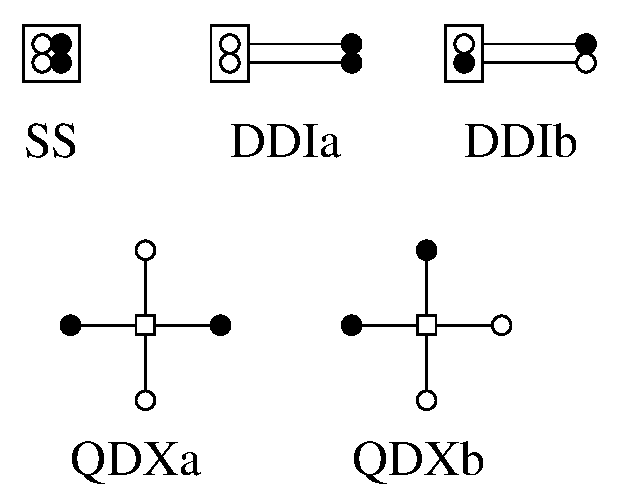
\includegraphics[scale=0.8]{figures/tetraquark_disp.pdf}
        \caption[Diagrammatic depiction of tetraquark displacements.]{Diagrammatic depiction of tetraquark displacements, taken from Ref.~\cite{spectroscopy}.}
        \label{fig:tetraquark_disp}
    \end{figure}
    \subsection{Projecting onto Symmetry Sectors}
    So far, we have outlined the construction of elemental single-hadron operators, which are indexed by Dirac spin, flavor, displacement, and momentum. The quantum numbers of interest on our periodic hypercubic lattice, however, are not Dirac spin, but the irreps of $O_h^D$, and in some circumstances, $G$-parity. We are therefore tasked with finding linear combinations of elemental hadron operators which create states possessing the relevant quantum numbers of the theory. That is, we find linear combinations
    \begin{equation}\label{eq:op_proj}
        \begin{aligned}
            \mathcal O_l(t) &= c^{(l)}_{\alpha\beta...}\Phi^{AB...}_{\alpha\beta...}(\bs p, t), \\
            \overline{\mathcal O}_l(t) &= c^{(l)*}_{\alpha\beta...}\overline\Phi^{AB...}_{\alpha\beta...}(\bs p, t),
        \end{aligned}
    \end{equation}
    where $l$ labels the relevant quantum numbers of the theory, and the projection coefficients $c^{l}_{\alpha\beta...}$ must be determined.

    Finding an operator which creates or annihilates a state with a given quantum number is equivalent to finding an operator that transforms according to the irreducible representation of a symmetry group. The particular irreducible representation is denoted by the quantum number $\Lambda$. We say that an annihilation operator $\mathcal O^{\Lambda \lambda}$ and its 
    corresponding creation operator $\overline{\mathcal O}^{\Lambda \lambda}$ transform according to the $\lambda$ row of the $\Lambda$ irreducible representation of a symmetry transformation $R$ when they satisfy
    \begin{equation}
        U_R \mathcal O^{\Lambda \lambda} U_R^\dagger = \sum_\mu \mathcal O^{\Lambda \mu} \Gamma_{\mu \lambda}^{(\Lambda)}(R)^*
    \end{equation}
    and
    \begin{equation}
        U_R \overline{\mathcal O}^{\Lambda \lambda} U_R^\dagger = \sum_\mu \overline{\mathcal O}^{\Lambda \mu} \Gamma_{\mu \lambda}^{(\Lambda)}(R),
    \end{equation}
    where $U_R$ is the unitary quantum operator associated with $R$, $\Gamma^{(\Lambda)}(R)$ is the matrix of the symmetry transformation $R$ in the $\Lambda$ irreducible representation.

    Given a general annihilation operator $\mathcal O$, we can can construct an operator $\mathcal O^{\Lambda \lambda}$ that transforms irreducibly using the following~\cite{spectroscopy}:
    \begin{equation}\label{eq:op_proj2}
        \mathcal O^{\Lambda \lambda} = \frac{d_\Lambda}{g_\mathcal G}\sum_{R\in \mathcal G} \Gamma^{(\Lambda)}_{\lambda \mu}(R) U_R \mathcal O U_R^\dagger
    \end{equation}
    where $d_\Lambda$ is the dimension of $\Lambda$, $R$ are the elements of the group $\mathcal G$, $g_{\mathcal G}$ is the order of $\mathcal G$, and all other quantum number indices have been suppressed. The index $\mu$ is arbitrary, though choosing $\mu = \lambda$ guarantees idempotency ($P^2=P$), making it a true projection. It is also important to note that Eq.~(\ref{eq:op_proj2}) does not uniquely specify the weights and the phases of the operators. This is important, because if we strategically set the relative normalizations of operators of different rows within an irrep, then it can be shown that the two-point correlation functions do not depend on irrep row. That is, it can be shown that in the absence of external degeneracy-breaking fields,
    \begin{equation}
        \bra{0}T \mathcal{O}_i^{\Lambda \lambda F}(t) \overline{\mathcal O}_j^{\Lambda \lambda F}(0)\ket{0} = \bra{0}T \mathcal{O}_i^{\Lambda \mu F}(t) \overline{\mathcal O}_j^{\Lambda \mu F}(0)\ket{0},
    \end{equation}
    where $\Lambda$ denotes octahedral irrep, $\lambda$ denotes irrep row, $F$ denotes all other quantum numbers, and $i$ \& $j$ index different operators in the $\Lambda\lambda F$ symmetry sector. Ultimately, this allows us to increase the statistics of our correlator measurements without the need of generating more gauge configurations, as we will see in Chapter~\ref{ch:montecarlo}.
    
    The details of obtaining the projection coefficients in Eq.~(\ref{eq:op_proj}) using the methods outlined here are given in Ref.~\cite{Basak:2005aq}.
    \section{Two-Hadron Operator Construction}
    In order to study scattering and resonance phenomena, it is necessary to probe the spectrum in the region of two-particle energies. This requires the use of operators which create states having overlap onto two-particle states. However, (in this work) we only study the spectrum up to three-particle energy thresholds, and therefore do not design operators to create states with more than two particles. This is because methods currently available to study scattering phenomena on the lattice (e.g.~the method of L\"uscher~\cite{Luscher:1990ck}) are only rigorously valid for energies that lie below three-particle thresholds.

    Once we have projected a single-hadron operator onto the relevant symmetry sectors, we are left with operators which can be written as $\mathcal O_{\bs p \Lambda \lambda i}^{I I_3 S}$ and its barred counterpart, where the relevant quantum numbers are isospin $I$, isospin projection $I_3$, strangeness $S$, momentum $\bs p$, octahedral irrep $\Lambda$, and octahedral irrep row $\lambda$. All other relevant labels (e.g.\ $G$-parity or displacement type), labeled by the compound index $i$.
    
    In order to form a final two-hadron operator, we start with a basis of products of single-hadron operators, as
    \begin{equation}
        \mathcal O_{\bs {p_a} \Lambda_a \lambda_a i_a}^{I_a I_{3a} S_a} \mathcal O_{\bs {p_b} \Lambda_b \lambda_b i_b}^{I_b I_{3b} S_b}.
    \end{equation}
    These products themselves do not transform irreducibly under isospin, $G$-parity (when relevant), or the octahedral symmetry group. In order to find linear combinations of these operator products which transform irreducibly under these symmetry groups, we simply use the same group-theoretical projection scheme presented in the previous section.

    As a final note, it is important to note the difference between a tetraquark operator and a two-meson operator. A two-meson operator is constructed by separately projecting two elemental meson operators onto individual symmetry sectors in order to form two final single-meson operators, and then projecting the product of the two single-meson operators onto the final desired symmetry sector. A tetraquark operator, on the other hand, is constructed by projecting a single elemental tetraquark operator (containing four quark fields) directly onto the final desired symmetry sector.